\documentclass[a4paper,14pt]{extreport} % формат документа

\usepackage{amsmath}
\usepackage{cmap} % поиск в ПДФ
\usepackage[T2A]{fontenc} % кодировка
\usepackage[utf8]{inputenc} % кодировка исходного текста
\usepackage[english,russian]{babel} % локализация и переносы
\usepackage[left = 2cm, right = 1cm, top = 2cm, bottom = 2 cm]{geometry} % поля
\usepackage{listings}
\usepackage{graphicx} % для вставки рисунков
\usepackage{amsmath}
\usepackage{float}
\usepackage{multirow}
\graphicspath{{img/}}
\DeclareGraphicsExtensions{.pdf,.png,.jpg}
\newcommand{\anonsection}[1]{\section*{#1}\addcontentsline{toc}{section}{#1}}

\lstset{ %
	language=Lisp,                % Язык программирования 
	numbers=left,                   % С какой стороны нумеровать          
	frame=single,                    % Добавить рамку
}

\begin{document}
\begin{titlepage}

    \begin{table}[H]
        \centering
        \footnotesize
        \begin{tabular}{cc}
            \multirow{8}{*}{
\includegraphics[scale=0.35]{bmstu.jpg}}
            & \\
            & \\
            & \textbf{Министерство науки и высшего образования Российской Федерации} \\
            & \textbf{Федеральное государственное бюджетное образовательное учреждение} \\
            & \textbf{высшего образования} \\
            & \textbf{<<Московский государственный технический} \\
            & \textbf{университет имени Н.Э. Баумана>>} \\
            & \textbf{(МГТУ им. Н.Э. Баумана)} \\
        \end{tabular}
    \end{table}

    \vspace{-2.5cm}

    \begin{flushleft}
        \rule[-1cm]{\textwidth}{3pt}
        \rule{\textwidth}{1pt}
    \end{flushleft}

    \begin{flushleft}
        \small
        ФАКУЛЬТЕТ
        \underline{<<Информатика и системы управления>>\ \ \ \ \ \ \ 
        \ \ \ \ \ \ \ \ \ \ \ \ \ \ \ \ \ \ \ \ \ \ \ \ \ \ \ \ \ \ \ 
    \ \ \ \ \ \ \ \ \ \ \ \ \ \ \ } \\
        КАФЕДРА
        \underline{<<Программное обеспечение ЭВМ и
        информационные технологии>>
        \ \ \ \ \ \ \ \ \ \ \ \ \ \ \ \ \ \ \ \ }
    \end{flushleft}

    \vspace{2cm}

    \begin{center}
        \textbf{Лабораторная работа № 1} \\
        \vspace{0.5cm}
    \end{center}

    \vspace{4cm}

    \begin{flushleft}
        \begin{tabular}{ll}
            \textbf{Дисциплина} & Экономика программной инженерии.  \\
            \textbf{Тема} & Планирование программного проекта в \\ 
            & Microsoft Project: настройка рабочей среды и \\
            & создание нового проекта.  \\
            \\
            \textbf{Студент} & Сусликов Д.В. \\
            \textbf{Группа} & ИУ7-85Б \\
            \textbf{Оценка (баллы)} & \\
            \textbf{Преподаватель} & Барышникова М.Ю., Силантьева А.В.   \\
        \end{tabular}
    \end{flushleft}

    \vspace{4cm}

   \begin{center}
        Москва, 2022 г.
    \end{center}

\end{titlepage}

\begin{enumerate}
\item \textbf{Тренировочное задание}

Вариант 2.

Начало: 01.03.22 г.

Конец: 13.05.22 г. 

Продолжительность: 51 день

\begin{figure}[H]
  \centering
  \caption{Тренировочное задание. }
  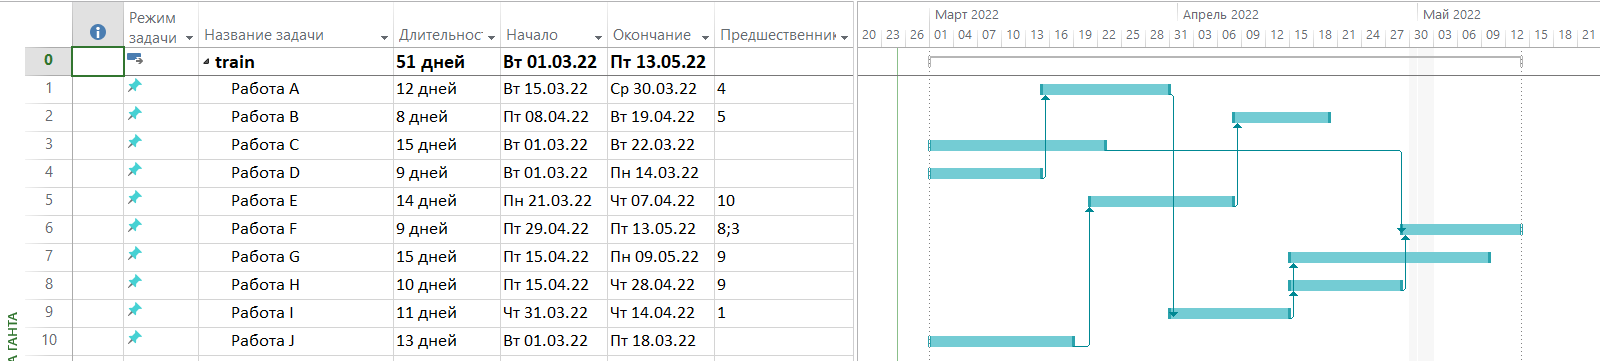
\includegraphics[scale=0.5]{dop}
\end{figure}

В календаре были заданы праздники и переносы до ноября 2022 года. Рабочий день длился 8 часов, с 9 до 18.
Тип задач -- фиксированный объем ресурсов.

\item \textbf{Основное задание}

Содержание проекта: Команда разработчиков из 16 человек занимается созданием карты города на основе собственного модуля отображения. Проект должен быть завершен в течение 6 месяцев. Бюджет проекта: 50 000 рублей.

\item \textbf{Задание 1}

Настройка рабочей среды проекта.

В настройках параметром, устанавливаем необходимое:
\begin{itemize}
\item Дата начала проекта – первый рабочий день марта текущего года.
\item Длительность работы в неделях, объем работ в часах, а тип работ -- с фиксированными трудозатратами.
\item Количество рабочих часов в день -- 8, количество рабочих часов в неделю -- 40.
\item Начало рабочей недели в понедельник, а финансового года - в январе.
\item Продолжительность рабочего дня с 9 до 18 часов.
\end{itemize}

\begin{figure}[H]
  \centering
  \caption{Настройка параметров. }
  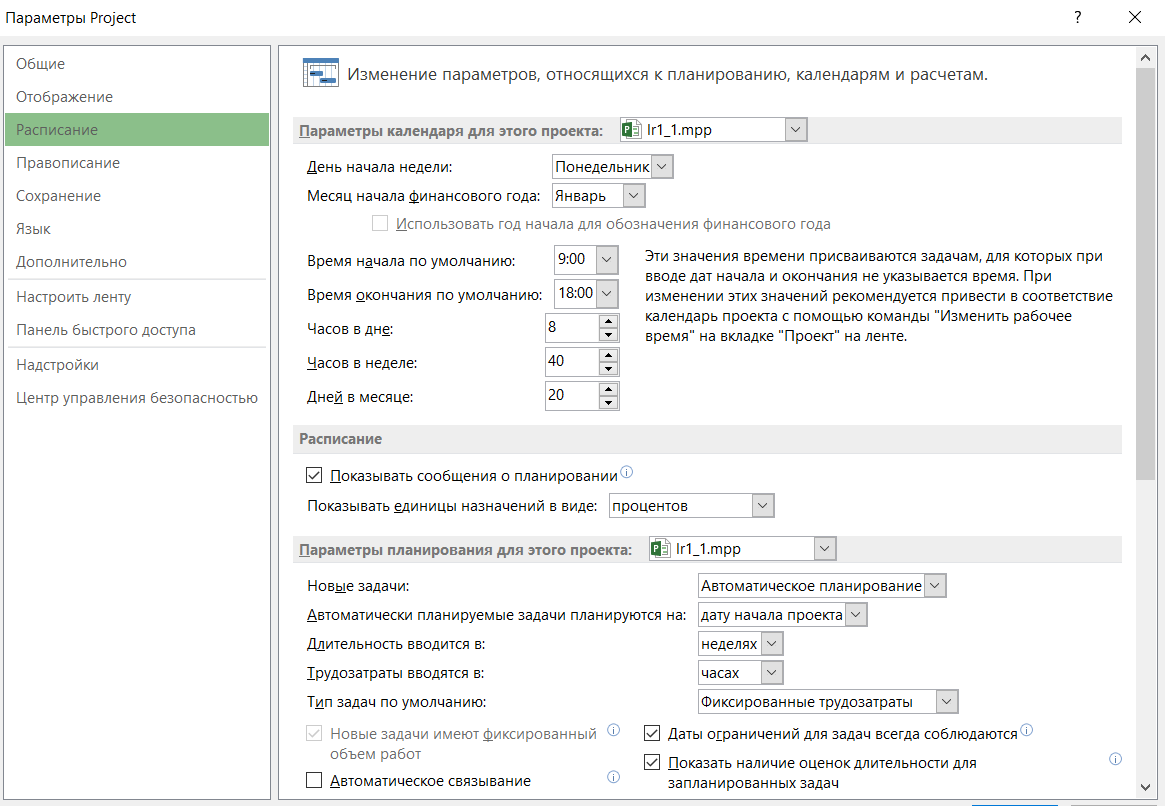
\includegraphics[scale=0.48]{calendar}
\end{figure}

Были отмечены выходные и праздничные дни на ближайшие календарные месяцы от даты начала проекта.

\begin{figure}[H]
  \centering
  \caption{Добавление выходных и праздников. }
  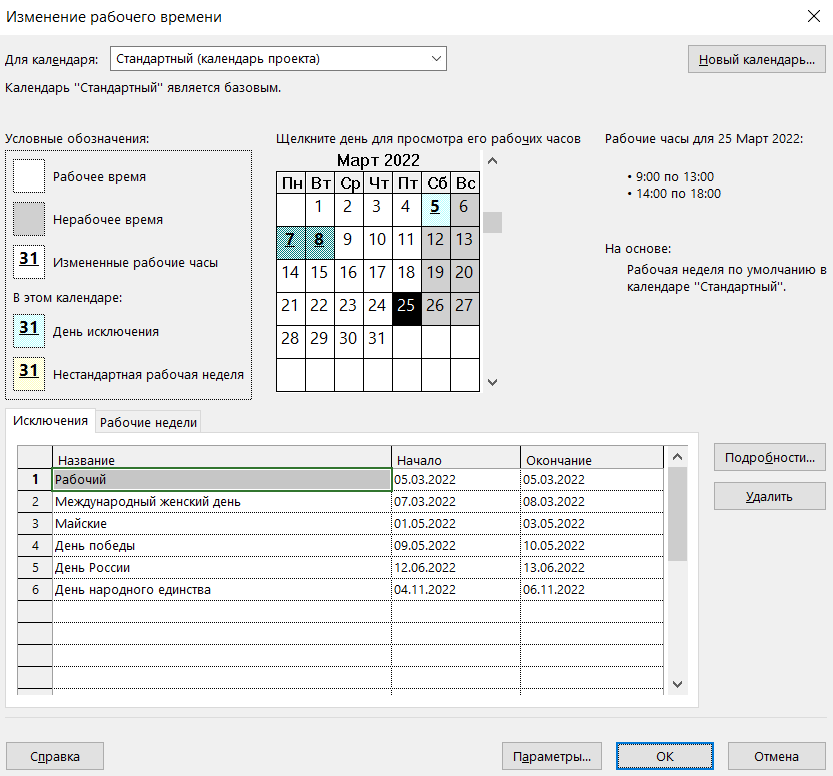
\includegraphics[scale=0.48]{holiday}
\end{figure}

Добавлена суммарная задача проекта и заметка с краткой информацией о нем.

\begin{figure}[H]
  \centering
  \caption{Суммарная задача и заметка. }
  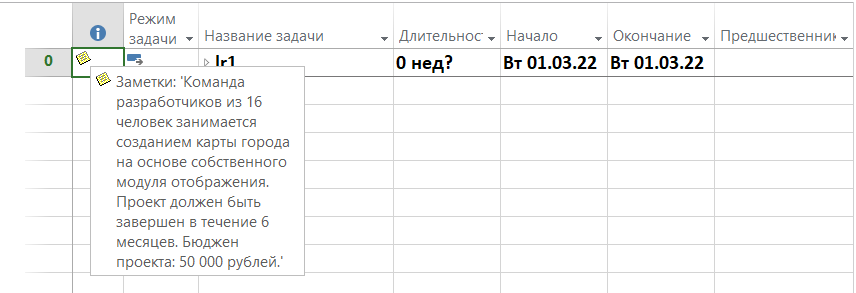
\includegraphics[scale=0.7]{note}
\end{figure}

\item \textbf{Задание 2}

Вводим список задач, в соотвествии с заднной таблицей.

Задачи 1 и 27 являются задачами вехами, они обозначают начало или конец фазы проекта и имеют нулевую продолжительность.

Задачи 2, 3, 8, 12,19 и 22 будут преобразованы в фазы проекта, поэтому длительность для них не указываем.

\begin{figure}[H]
  \centering
  \caption{Список задач. }
  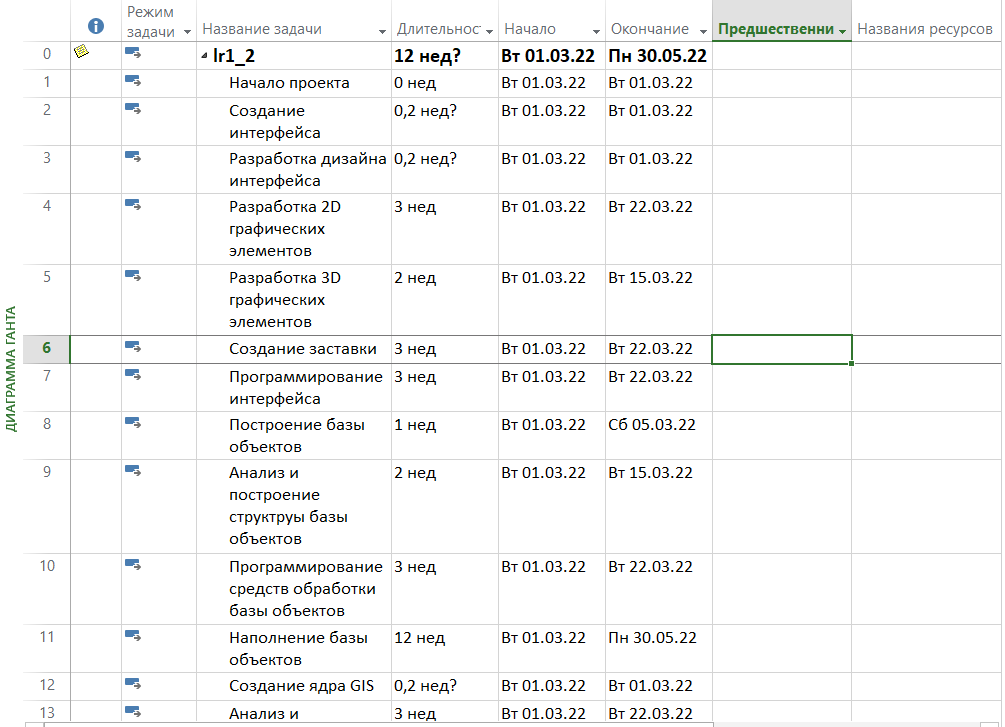
\includegraphics[scale=0.8]{11}
\end{figure}

\begin{figure}[H]
	\centering
	\caption{Список задач. }
	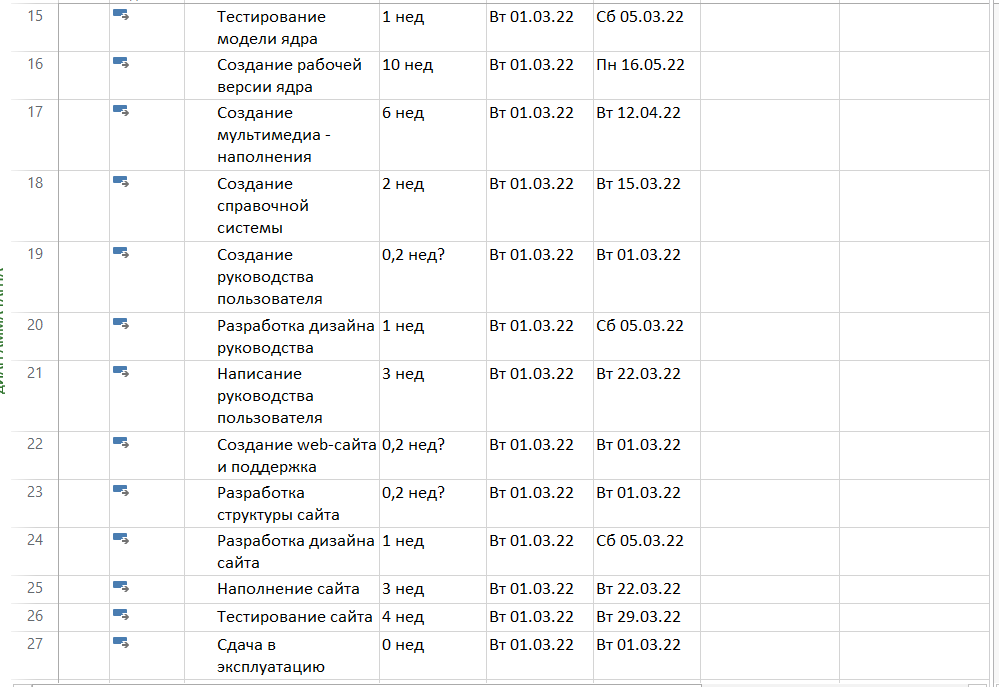
\includegraphics[scale=0.8]{12}
\end{figure}

\item \textbf{Задание 3}

Далее группируем задачи как подзадачи -- структурируем список. 

\begin{figure}[H]
  \centering
  \caption{Структурирование списка задач. }
  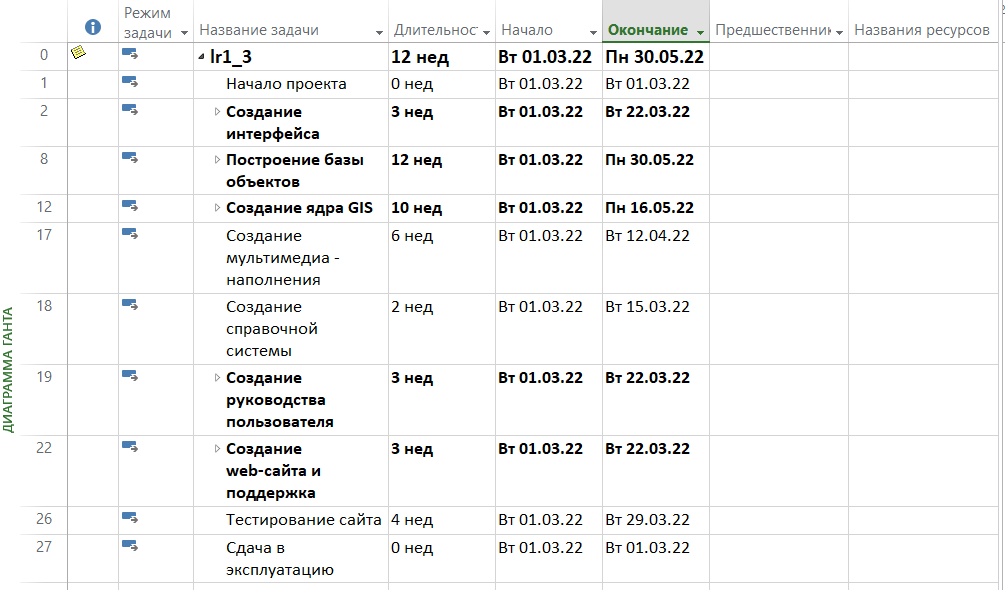
\includegraphics[scale=0.8]{2}
\end{figure}

\item \textbf{Задание 4}

Далее связываем задачи между собой: НН -- задачи начинаются одновременно, ОН -- задача начинается после окончания предыдущей. Также можно ввести запаздывание -- положительное число и опережение -- отрицательное число.

\begin{figure}[H]
  \centering
  \caption{Установление связей между задачами. }
  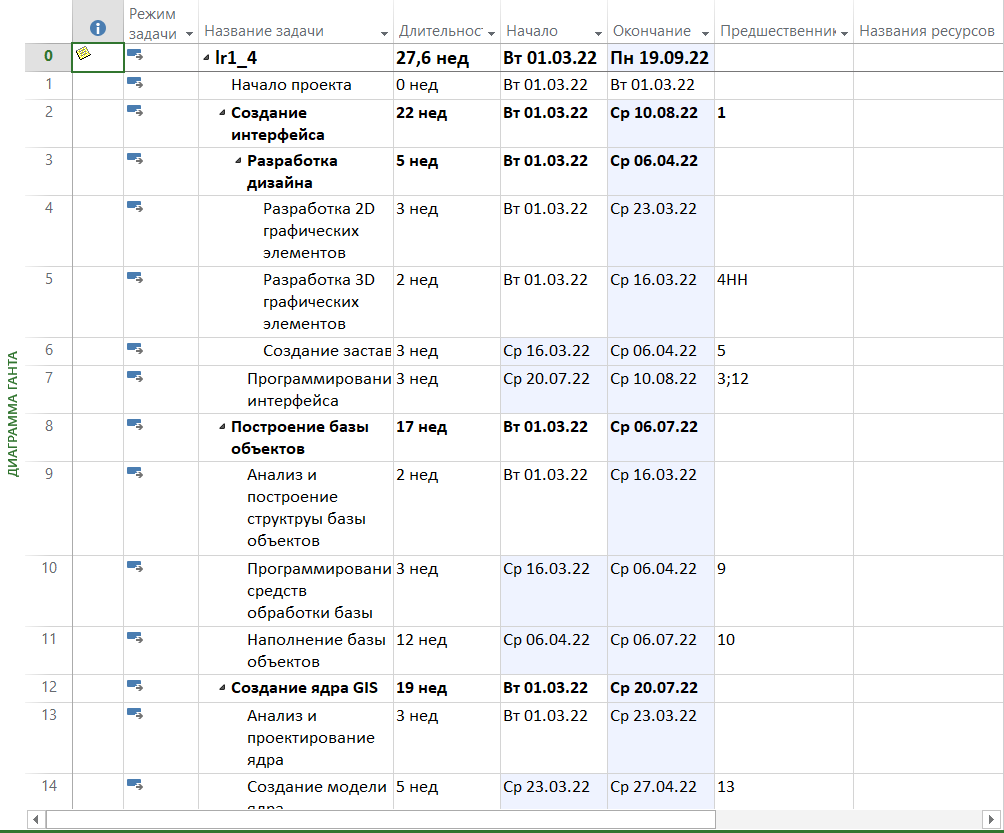
\includegraphics[scale=0.8]{31}
\end{figure}

\begin{figure}[H]
	\centering
	\caption{Установление связей между задачами. }
	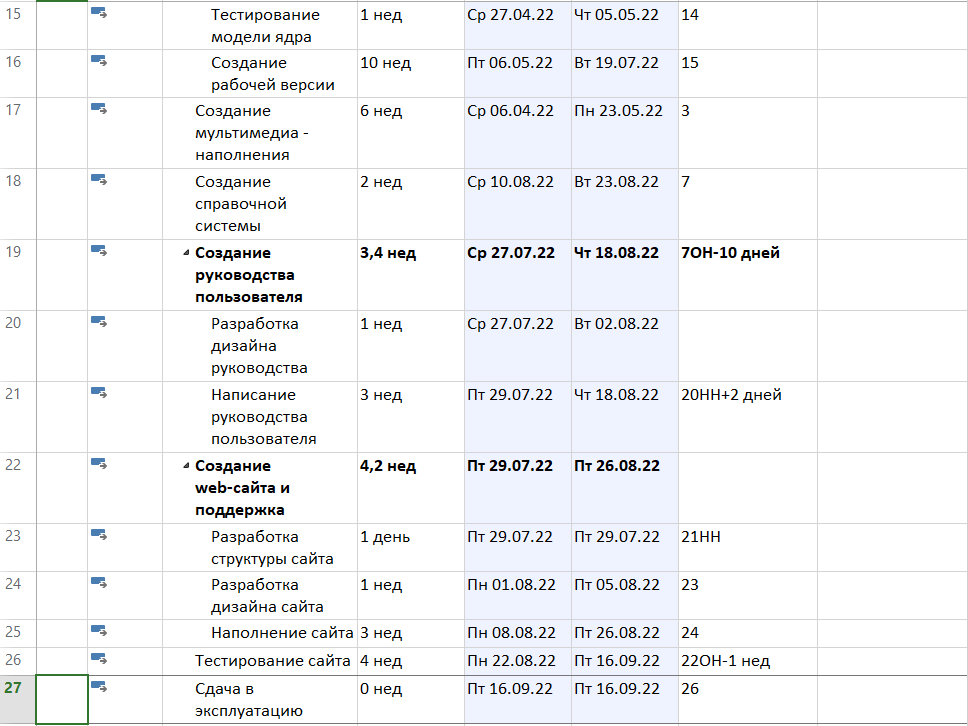
\includegraphics[scale=0.8]{32}
\end{figure}

\newpage

\item \textbf{Вывод}

В ходе выполнения лабораторной работы были изучены возможности программы Microsoft Project 2013. Была проведена настройка рабочей среды, создание списка задач, их структурирование и установление связей между ними.

В результате установлено, что несмотря на то, что на проект было заложено 6 месяцев, он не будет завершен вовремя. По проведенному анализу было выяснено, что ориентировочная дата завершения – 19 сентября (срок исполнения -- 27.6 недель).

\end{enumerate}

\end{document}